\documentclass[12pt]{article}

% Packages for title page
\usepackage{graphicx} % For including images
\usepackage{titling} % For modifying the title
\usepackage{datetime} % For including date and time
\usepackage{geometry}
 \geometry{
 a4paper,
 left=20mm,
 top=20mm,
 }

% Packages for table of contents
\usepackage{tocloft} % For modifying the table of contents

% Packages for main content
\usepackage{lipsum} % For generating placeholder text
\usepackage{hyperref} % For creating hyperlinks

% Set up title page
\pretitle{\begin{center} \LARGE 
\includegraphics[width=0.5\linewidth]{tulogo.png}\\[\bigskipamount]\end{center}}
\posttitle{}

\title{ \begin{center} \LARGE Vehicle Accident Prevention System (VAPS) \end{center} }
\author{\\ \\Team Members: 
\\
\\
\\
Aman Kumar EEB20035\\
Apoorv Krishan EEB20034\\
Shabnam Ajaj EEB20025\\
Vicky Kumar EEB20043\\}
\date{}


% Set up table of contents
\setlength\cftbeforesecskip{0.5em} % Space between sections in the table of contents

\begin{document}

\maketitle
\newpage
\tableofcontents

\newpage

\section{Objective}
Our proposed project focuses on addressing the alarming issue of vehicle accidents, with a particular emphasis on heavy vehicles. The primary cause of these accidents is driver negligence, which most commonly manifests in the form of drowsy driving and driving under the influence of alcohol. The consequences of such accidents can be catastrophic, causing loss of life, property damage, and financial burden.
\\
\\
Therefore, our project aims to provide a comprehensive solution that not only tackles the problem of accidents but also streamlines the logistics process. We envision an end-to-end system that incorporates cutting-edge technologies to solve the problem. By leveraging these technologies, we can develop a solution that can accurately monitor drivers' behaviour and alert them in real-time if they exhibit signs of drowsiness or impairment.
\\
\\
Furthermore, our solution will incorporate intelligent law enforcement helping tools to help maintain the law and order on the roads. Our ultimate goal is to make the roads safer for everyone while improving the bottom line for logistics companies.

\section{Background}
The problem of vehicle accidents due to driver negligence, specifically drowsy and drunk driving, has become a growing concern worldwide. These accidents result in significant loss of life, property damage, and financial burden. Despite the implementation of strict laws and regulations, many drivers continue to engage in these unsafe practices, leading to preventable accidents.
\\
\\
Current solutions to address this problem, such as random breath testing and driver education programs, have limitations in terms of effectiveness and scalability. Furthermore, these solutions do not provide real-time feedback to drivers, leaving room for human error and increasing the risk of accidents.
\\
\\
To address these issues, we propose the use of Arduino and sensors to detect drowsiness and drunk driving in real time. This solution has the potential to significantly reduce the number of accidents caused by driver negligence, making driving safer and more efficient. However, the development of such a system requires careful consideration and planning to ensure that it is reliable, accurate, and cost-effective.
\\ 
\\
Therefore, the problem statement for our proposed project is to design and develop a comprehensive system using Arduino and sensors that can accurately detect drowsiness and drunk driving in real-time, providing feedback to drivers to prevent accidents caused by driver negligence.

\section{Component Description}

\subsection{Arduino}
Arduino is an open-source electronics platform based on easy-to-use hardware and software. It is designed for artists, designers, hobbyists, and anyone interested in creating interactive objects or environments. The platform consists of a programmable microcontroller, a software development environment, and a community of users and developers who share their projects and code.
\\
\\
\\
\\
We can send a programme to the Arduino board that contains a set of instructions that can perform simple to complex tasks. Traditional programmable circuit boards necessitate the use of additional hardware to load the code onto the board. However, Arduino eliminates the need for hardware by loading code onto the Arduino board using a simple USB cable.The Arduino board enables developers to feed the program in the simplified version of the C++ language, making it easier for them to learn and code. 
\\
\\

The Arduino Uno employs an ATmega328P microcontroller from the 8-bit AVR family, which functions at a 5 Volt level. The suggested input voltage range is 7-12V, while the acceptable range is between 6-20V. The device has six analog input pins labeled A0-A5 and fourteen digital input/output pins, six of which provide Pulse Width Modulation (PWM) output. The maximum DC current that the I/O pins can handle is 40mA, while the 3.3V pin can handle 50mA. The device has 32KB of Flash memory, 0.5KB of which is reserved for the bootloader, 2KB of Static Random Access Memory (SRAM), and 1KB of Electrically Erasable Programmable Read-Only Memory (EEPROM). The device's operating frequency is 16MHz.
\\
\\
\\
\subsubsection{Arduino Hardware}
The Arduino's programmable circuit board is its hardware component. In our work, we have come across a variety of Arduino boards, but the most commonly used Arduino board is the Arduino UNO. The heart of the Arduino platform is the microcontroller, which is a small computer on a single integrated circuit. The microcontroller is programmed using the Arduino software development environment, which is based on the Processing programming language. The software development environment includes a code editor, a compiler, and a bootloader that allows the code to be uploaded to the microcontroller.
\\
\\
Arduino boards are available in a variety of form factors, including the Uno, Mega, Nano, and Due. These boards differ in their features and capabilities, but all are based on the Atmel AVR microcontroller. The boards typically include a USB interface for programming and serial communication, digital and analog input and output pins, and other features such as timers, interrupts, and communication interfaces.
\\
 \\
\subsubsection{Arduino Software}
The Arduino software development environment is a cross-platform software tool that is used to create, upload, and debug Arduino sketches. It is based on the Processing programming language, which is designed to make programming more accessible to artists and designers. The software development environment includes a code editor, a compiler, and a bootloader that allows the code to be uploaded to the microcontroller. The code editor provides syntax highlighting and autocompletion features that make it easier to write code. The compiler converts the code into machine language that the microcontroller can understand. The bootloader is a small piece of code that runs on the microcontroller when it is first powered on, and it allows the microcontroller to be programmed over a serial connection.
\\
\\
One of the key features of the Arduino platform is its ease of use. The software development environment and programming language are designed to be simple and accessible to beginners, while still providing powerful features for advanced users. This low cost, combined with the platform's ease of use, has made it a popular choice for educational purposes, as well as for hobbyists and professional designers.
 \\
 \\
\subsubsection{Arduino Programming}
Arduino programming is done using a high-level programming language that is similar to C and C++. The language includes a set of standard functions and libraries that make it easy to interact with the microcontroller's input and output pins, as well as other peripherals such as serial communication ports and timers. Arduino programming also includes support for interrupts, which allows the microcontroller to respond to external events in real-time.
\\
\\
Aside from hardware and software, the code, also known as a sketch, is the third most important aspect of Arduino. The code can be written in the Arduino IDE and loaded onto the board. The Arduino Programming Language is a native language similar to C++. Any programme written in the Arduino Programming Language is referred to as a sketch and is saved in a file with the.ino extension.
Arduino is made up of hardware, software, and code.
\\
\\
Overall, Arduino provides a powerful and accessible platform for creating interactive electronics projects. Its ease of use, low cost, and community support make it an ideal choice for hobbyists and professionals alike. Whether you are interested in robotics, home automation, or art installations, Arduino provides a flexible and powerful platform for bringing your ideas to life.
\\
\\
\subsection{IR Sensor}
An IR sensor, or infrared sensor, is a type of electronic component that detects infrared radiation. Infrared radiation is a form of electromagnetic radiation that has a longer wavelength than visible light and is typically emitted by heat sources. IR sensors are commonly used in a variety of applications, including remote controls, motion sensors, and temperature sensors.
\\    
\\
\subsubsection{Operation}
The basic operation of an IR sensor involves detecting changes in the intensity of infrared radiation. The sensor consists of an infrared emitter and an infrared detector, which are typically housed in a single package. The emitter generates infrared radiation, which is directed toward the object or area being monitored. The detector measures the intensity of the infrared radiation that is reflected or emitted by the object, and generates a signal that is proportional to the intensity.
\\
\\
An IR LED is a type of transmitter that emits infrared radiation. This LED appears to be a standard LED, and the radiation it emits is not visible to the naked eye. Infrared receivers detect radiation primarily through the use of an infrared transmitter. Infrared receivers are available as photodiodes. IR Photodiodes differ from conventional photodiodes in that they only detect IR radiation. There are various types of infrared receivers based on voltage, wavelength, package, and so on.
\\
\\
When used in conjunction with an IR transmitter and receiver, the wavelength of the receiver must equal that of the transmitter. The transmitter in this case is an IR LED, and the receiver is an IR photodiode. The infrared photodiode is sensitive to infrared light emitted by an infrared LED. The resistance of the photodiode and the change in output voltage are proportional to the amount of infrared light obtained.
\\
\\
\subsubsection{Uses}
IR sensors can be used in a variety of applications, including temperature sensing, motion detection, and remote control. In temperature sensing applications, IR sensors can be used to measure the temperature of objects without physically touching them. This is particularly useful in applications where contact temperature sensing may be impractical or unsafe, such as in medical devices or industrial settings.
\\
\\
In motion detection applications, IR sensors can be used to detect the movement of people or objects. This is accomplished by detecting changes in the intensity of infrared radiation in the environment. Motion sensors are commonly used in security systems and home automation applications.
\\
\\
In remote control applications, IR sensors are used to receive signals from a remote control device, such as a television remote or a garage door opener. The sensor detects the infrared radiation emitted by the remote control and translates it into a control signal that can be used to operate a device.
\\
\\
There are two types of infrared sensors: active and passive. 

\subsubsection{Active infrared sensors}
An active IR sensor is a type of infrared sensor that emits infrared radiation and then detects the reflected radiation to determine the presence or absence of an object or the distance to the object. Unlike passive IR sensors, which detect changes in the heat emitted by objects, active IR sensors emit their own IR radiation and then measure the reflection to detect the presence of an object.Active IR sensors are commonly used in proximity sensors, distance measuring devices, and object detection systems. They are also used in automation and robotics applications to detect the presence of objects and to assist in navigation.
\\
\\
The basic operation of an active IR sensor involves emitting a short pulse of infrared radiation and then measuring the time it takes for the reflection to return to the sensor. This time delay is used to determine the distance to the object being detected. The sensor may use a variety of different methods to emit the IR radiation, such as an LED or a laser diode.
\\
\\
One of the advantages of active IR sensors is their ability to detect objects in low light conditions. Because the sensor emits its own IR radiation, it is not dependent on ambient light to detect the presence of objects. This makes active IR sensors well-suited for use in environments with low levels of ambient light, such as dark rooms or outdoor environments at night.
\\
\\
Another advantage of active IR sensors is their ability to provide accurate distance measurements. By measuring the time it takes for the reflected IR radiation to return to the sensor, active IR sensors can provide highly accurate distance measurements. This makes them well-suited for use in applications where precise distance measurements are required, such as in robotics and automation applications.
\\
\\
Overall, Active IR sensors are a powerful and versatile type of sensor that are well-suited for a wide range of applications. They are particularly useful in proximity sensing, distance measuring, and object detection applications. While there are challenges associated with using active IR sensors, such as interference from other sources of IR radiation, these challenges can be overcome with proper design and implementation.
\\
\\
\subsection{MQ3 Alcohol Sensor}
The MQ3 alcohol gas sensor module detects alcohol, CH4, benzene, petrol, hexane, CO, and LPG. It has a sensitive material SnO2 for detecting alcohol gas, with lower electrical conductivity in fresh air. It is a semiconductor alcohol gas sensor that detects or monitors alcohol presence or absence. It is also referred to as a chemiresistor because the sensing of the sensitive material is based on the resistance change when the sensor is exposed to alcohol gas.
\\
\\
The MQ3 Alcohol Sensor requires a power supply of 5VDC, consuming 165mA when the heater is ON and 60mA when it's OFF. The current is 150mA, and the digital output is TTL digital, represented by 0 and 1, which translates to 0.1V and 5V, respectively. The analog output ranges from 0.1V to 0.3V and correlates to the degree of pollution, voltage concentration, and has a maximum value of 4V. The sensor can detect alcohol concentration levels from 0.05 mg/L to 10 mg/L. Its interface consists of one TTL compatible input (HSW) and one TTL compatible output (ALR). The heater's power consumption is 750mW, and its resistance is 33ohms±5 percent. The device can operate within the temperature range of -10°C to 50°C (14°F to 122°F) and can be stored within the temperature range of 20°C to 70°C. The load resistance of the sensor is 200kilo ohms, and its sensitivity Rs is 5: Rs(in the air) / Rs(0.4mg/L Alcohol). The sensing resistance Rs ranges from 1Mega ohms to 8Mega ohms at 0.4mg/L alcohol concentration. The sensor's dimensions are 32x22x16mm, and its humidity must remain below 95 percent RH, while the oxygen concentration should remain at 21%. The slope rate is 0.6, and the preheating duration is 20 seconds.
\\
\\
The SnO2 conductivity increases as the sensor is moved closer to the alcohol gas. The increase in sensor conductivity is proportional to the concentration of alcohol. As a result, any microcontroller can easily measure the alcohol concentration. The MQ3 alcohol gas sensor is extremely fast and sensitive to alcohol, smoke and petrol. This alcohol sensor can be used to create an alcohol detector.
\\
\\
The MQ3 Alcohol Sensor is commonly used in breathalyzer devices, which are used to measure the blood alcohol content (BAC) of individuals who may be driving under the influence of alcohol. The sensor can also be used in other applications where alcohol detection is required, such as in industrial settings where alcohol is used as a solvent or in the production of beverages.
\\
\\
\subsubsection{Working}
The MQ3 Alcohol Sensor operates on a supply voltage of 5V DC and consumes approximately 150mA of current during operation. The sensor's output is an analog voltage signal that varies with the concentration of alcohol in the air. The output voltage range is typically between 0.4V and 2V, with higher voltages indicating higher concentrations of alcohol.
\\
\\
The MQ3 Alcohol Sensor module is sensitive to other gases besides alcohol, so it is important to calibrate the sensor before use to ensure accurate measurements. Calibration involves exposing the sensor to a known concentration of alcohol vapors and adjusting the module's circuitry to compensate for any cross-sensitivity to other gases. The MQ3 sensor's alcohol gas sensing range in fresh air or atmosphere is 0.04mg/L-4 mg/L, which is suitable for breathalysers. It draws 150 mA and runs on a 5V power supply in temperatures ranging from -10°C to 50°C.
\\
\\
The MQ3 Alcohol Sensor module can be interfaced with a microcontroller or other electronic device using analog or digital inputs. Many microcontroller platforms, such as Arduino, have libraries and examples available for interfacing with the MQ3 Alcohol Sensor module.
\\
\\
One of the challenges of using the MQ3 Alcohol Sensor is that its response time can vary depending on a number of factors, such as the concentration of alcohol in the air and the temperature of the sensor. To achieve accurate and reliable measurements, it is important to allow the sensor to warm up and stabilize before taking measurements, and to account for any variation in response time when interpreting the sensor's output.
\\
\\
Overall, the MQ3 Alcohol Sensor is a powerful and versatile gas sensor module that is well-suited for detecting alcohol vapors in the air. With its low power consumption and simple interface, the MQ3 Alcohol Sensor is ideal for a wide range of applications, from breathalyzer devices to industrial process monitoring. However, it is important to carefully calibrate and account for the sensor's response time and cross-sensitivity to other gases to ensure accurate and reliable measurements.
\\
\\
\subsection{Bluetooth BLE Module}
Bluetooth Low Energy (BLE) is a wireless communication technology that is designed to consume very little power while maintaining a robust and reliable connection. BLE is a subset of the Bluetooth standard, and it is intended for use in devices that require low power consumption, such as wearable devices, health monitors, and other Internet of Things (IoT) devices.
\\
\\
The Bluetooth technology being used is version 2.0 + EDR, which stands for Enhanced Data Rate. The frequency used is in the 2.4 GHz ISM band, with a GFSK modulation method (Gaussian Frequency Shift Keying). The transmit power is classified as Class 2, with a maximum of 4 dBm. The typical sensitivity level is -80 dBm, and the range for open air is about 10 meters or 33 feet. Supported profiles include SPP (Serial Port Profile), HID (Human Interface Device), and others. The device operates within a voltage range of 3.3V to 5V DC, with less than 50mA of operating current, less than 2.5mA of standby current, and less than 1mA of sleep current. The device uses UART (Universal Asynchronous Receiver/Transmitter) as its interface, with a range of baud rates from 1200 to 460800. The device can operate within a temperature range of -20°C to 75°C (-4°F to 167°F).
\\
\\
\subsubsection{Operation}
The BLE module is a small electronic device that contains a Bluetooth chip and other electronic components that allow it to communicate with other devices over a Bluetooth connection. BLE modules typically operate in the 2.4 GHz frequency band, which is an unlicensed band that is used for a variety of wireless communication technologies. BLE devices use a frequency hopping scheme to avoid interference from other devices in the same frequency band.
\\
\\

BLE technology uses a master/slave architecture, where one device (the master) initiates the connection, and one or more devices (the slaves) respond to the master's requests. This allows the master device to control the communication between the devices and to conserve power by controlling when and how often the slaves transmit data.
\\
\\
BLE modules can be programmed using a variety of programming languages and development tools. Many BLE modules come with a software development kit (SDK) that includes libraries and examples for programming the device. BLE modules can also be programmed using Arduino or other microcontroller platforms, allowing developers to create custom applications and interfaces.
\\
\\
\subsubsection{Communication & Pairing}
BLE communication is based on a set of profiles and services, which define the types of data that can be exchanged between devices. Profiles are collections of services that define a particular type of device, such as a heart rate monitor or a temperature sensor. Services are collections of characteristics that define a particular type of data, such as heart rate or temperature. Characteristics can be read, written, or notified, allowing devices to exchange data in a variety of ways.
\\
\\
BLE communication is typically initiated through a process called pairing. Pairing is a secure process that allows two devices to establish a trusted connection. During pairing, the devices exchange encryption keys that are used to secure the communication between the devices. Once paired, the devices can exchange data securely and reliably.
\\
\\
\subsubsection{Advantages}
The main advantage of BLE technology is its low power consumption. BLE devices can operate for long periods of time on a single battery, making them ideal for devices that need to be portable or that require long-term monitoring. BLE devices are also designed to be highly reliable, with a robust connection that can work even in challenging environments.BLE modules can be integrated into a variety of devices, including sensors, medical devices, and home automation systems.
\\
\\
Overall, Bluetooth Low Energy (BLE) is a powerful and reliable wireless communication technology that is ideal for low-power, portable devices. BLE modules are easy to integrate into a variety of devices, and they offer a secure and reliable communication channel for exchanging data. With its low power consumption and robust connection, BLE technology is well-suited for a wide range of IoT applications, including wearable devices, medical devices, and home automation systems.
\\
\\
\section{Methodology}
The design and development of the solution can be divided into two parts: Hardware development and Software Development. 
\\ 
\\ 
The two parts are the essential parts for the working of the entire solution.  While the hardware part is essential for the interaction of the system with humans (driver) while the software part is the decision-maker and background assisting part of the system, which helps to streamline the solution as well as make it user-friendly and cheap. 

\begin{figure}[ht]

\centering
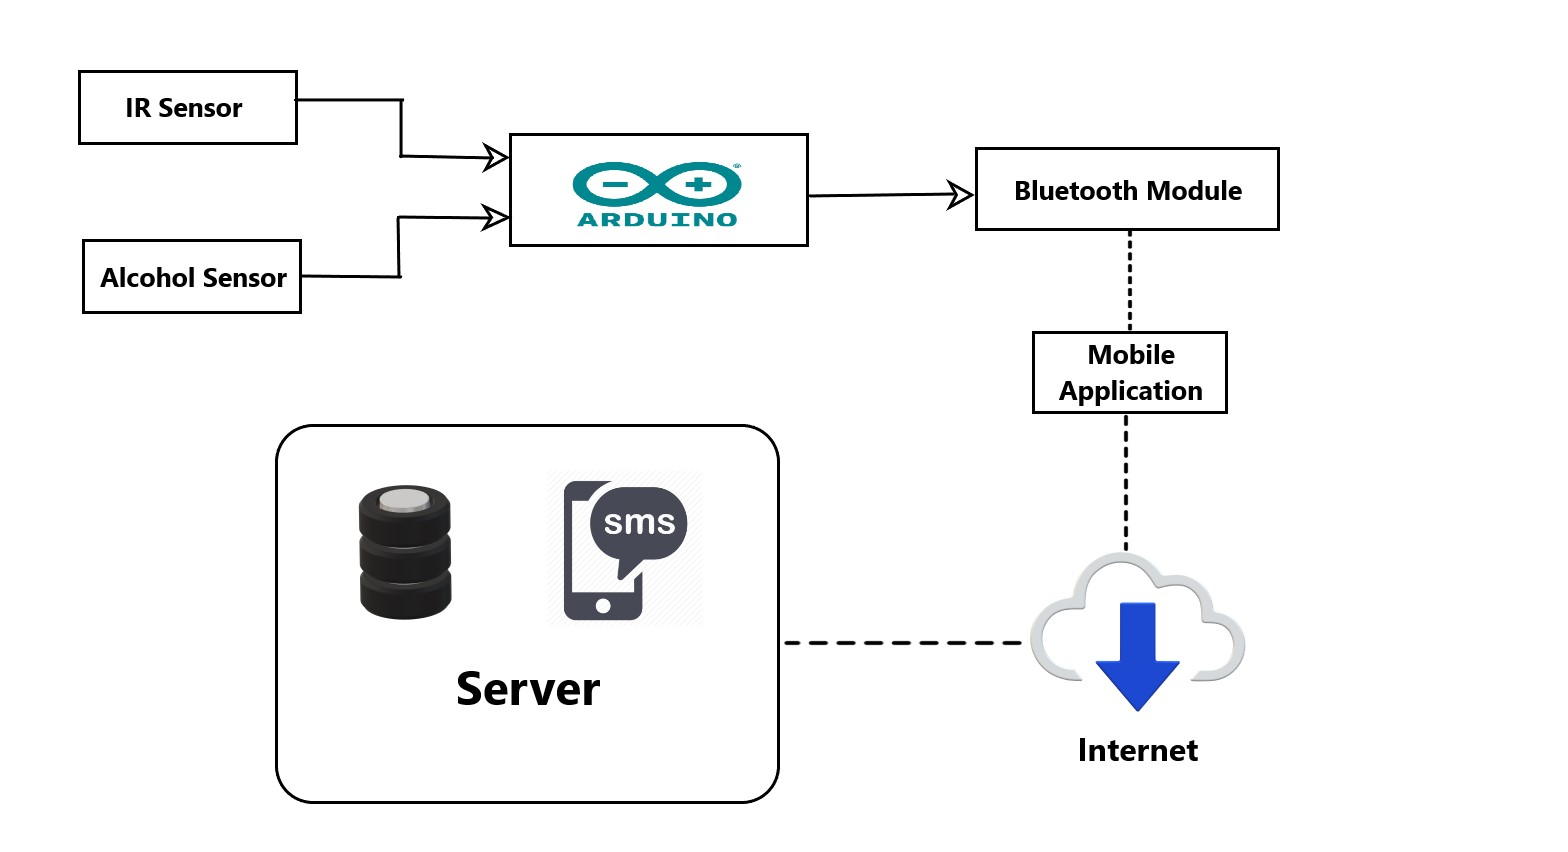
\includegraphics[width=\textwidth]{eld_report.jpg}
\caption{System Design of the proposed solution.}

\end{figure}

\subsection{Hardware Development}
The development of the hardware for the proposed solution includes the making of a spectacle to track drowsiness and alcohol consumption by the user (driver). This developed hardware solution will be employing a low-power, open-source device Arduino for onboard data processing, an infrared sensor (IR) for eye tracking and sleep detection, and an MQ3 Alcohol sensor for alcohol detection on board. 
\\
The Arduino, IR Sensor, Alcohol Sensor and the Bluetooth Module are connected to each other as per the circuit topology given in the \ref{fig:} . The IR sensors detects obstacle in general purpose use as it emits infrared and then receives back the reflected rays, the comparator on the IR Module compares the voltage generated using the IR receiver with the voltage drop across the potentiometer thus, setting a baseline voltage value using the potentiometer. This decides the distance to which the IR sensor can sense. In our case, the IR sensor is employed to sense the rays from the eye of the driver when a beam of infrared is transmitted through the IR transmitter. When eyes are opened the received value is low as no light is being reflected back while when when the eyes are closed, the closed eyelids reflects back a portion of infrared light back to IR receiver. This sends a output of 1 or digital high into the Arduino. Similarly, the MQ3 alcohol sensor senses the presence of alcohol and converts it into voltage value and based on the presence of the amount of alcohol detected and the base value set by the potentiometer, the comparator sends digital high or digital low output to the Arduino..
\\
Based on the output of the sensors, the Arduino sends a deli meter byte if 1 through the connected Bluetooth module. Subsequently. the Arduino is also used to generate a ignition trigger signal which is visualized in our model as an LED but can be used to various tasks in real-life application such as speed control, switching ion the hazard lights and applying brakes of the vehicle. 
\\
\\
\\
\\
This entire hardware assembly will be mounted on a glass frame for demonstration purposes but can also be made into a final product similarly. The Arduino will be connected to an HC-05 Bluetooth module that can be connected to the user's smartphone device via Bluetooth. 
\\
Along with that, the Arduino can be programmed to trigger a separate system that can reduce the vehicle speed as well as switch on the hazard lights to indicate the potential problem with the vehicle on the road. 
\\
\\
\subsection{Software Development}
As important is the hardware part in our proposed solution for the detection of anomalies in the driver behaviour, the software part is also similarly important to make this proposed solution cheap and effective. \\ \\ 
The Bluetooth module connected via Bluetooth to the user's smartphone device communicates with the app installed in the driver's app in the phone. The app waits for receiving a deli-meter byte and acts on its receivance. When a deli-meter byte is received on the app, it performs a couple of tasks starting with sending a SMS (), containing the location of the affected vehicle, to a specified phone number, generally the owner of the vehicle or the in charge of the vehicle.
\\
Second task it performs is the logging of data (latitude, longitude and the of anomaly) onto the online real-tie database that we have hosted using fire-base. The app was developed using MIT app inventer service that hepls in easy development of logical apps. 
\\
Another part of the system includes a online monitoring server that checks for the every new logged data and then finds the closest helpful service such as police vehicles, police stations etc. by comparing the latitude and longitude of the affected vehicle to the services in the database.
% \section{Results}
% \lipsum[4]

% \section{Discussion}
% \lipsum[5]


\section{Conclusion}
 Our proposed project aims to address the critical issue of driver negligence, specifically drowsy and drunk driving, which has become a growing concern worldwide. We recognize the severe consequences of such accidents, including loss of life, property damage, and financial burden, and believe that our end-to-end solution can help mitigate these risks. By leveraging cutting-edge technologies such as Arduino and sensors, we can develop a comprehensive system that can accurately monitor drivers' behavior and alert them in real-time if they exhibit signs of drowsiness or impairment. Furthermore, our solution will incorporate intelligent law enforcement tools to help maintain law and order on the roads, making the roads safer for everyone while keeping the logistics system safe from point failure. Although the development of such a system requires careful consideration and planning to ensure that it is reliable, accurate, and cost-effective, our proposed solution possesses great potential to reduce the number of accidents caused by driver negligence, making driving safer and more efficient.

% Add references section
% \section*{References}
% \addcontentsline{toc}{section}{References}

% Add references here
\section{Appendix}

\subsection{Component Specification}
\subsubsection{Arduino Uno}
\begin{tabular}{|c|c|}
    \hline
    COMPONENT & SPECIFICATION \\
    \hline
    Microcontroller & ATmega328P – 8 bit AVR family microcontroller \\
    \hline
    Operating Voltage & 5V \\
    \hline
    Recommended Input Voltage & 7-12V \\
    \hline
    Input Voltage Limits & 6-20V \\
    \hline
    Analog Input Pins & 6 (A0 – A5) \\
    \hline
    Digital I/O Pins & 14 (Out of which 6 provide PWM output) \\
    \hline
    DC Current on I/O Pins & 40 mA \\
    \hline   
    DC Current on 3.3V Pin & 50 mA \\
    \hline
    Flash Memory & 32 KB (0.5 KB is used for Bootloader) \\
    \hline
    SRAM &2 KB \\
    \hline
    EEPROM & 1 KB \\
    \hline
    Frequency (Clock Speed) & 16 MHz \\
    \hline
\end{tabular}
\subsubsection{IR Sensor}
\begin{tabular}{|l|l|l|l|l|}
\hline
Symbol & Quantity                 & Minimum & Maximum & Unit \\ \hline
o/p    & Output Voltage           & 0       & 5       & V    \\ \hline
Vcc    & Operating Voltage        & 4.5     & 5.5     & V    \\ \hline
GND    & Ground Reference Voltage & -       & -       & V    \\ \hline
\end{tabular}
\subsubsection{MQ3 Alcohol Sensor}
\begin{tabular}{|c|c|}
    \hline
     COMPONENT & SPECIFICATION  \\
    \hline
    power supply & 5VDC (@ 165mA heater ON / 60mA heater off). \\
    \hline
    Current & 150mA \\
    \hline
    Digital output Do& 0 and 1 TTL digital (0.1V and 5V).\\
    \hline
    Analog output Ao& 0.1V to 0.3V (relates to pollution), 
    \\ & voltage concentration and maximum of 4V.\\
    \hline
    Alcohol Concentration detection& 0.05 mg/L to 10 mg/L.\\
    \hline
    Interface& one TTL compatible input(HSW) and \\ & one TTL compatible output(ALR). 
    \\
    \hline
    Heater consumes& <750mW. \\
    \hline
    Resistance of the heater& 33ohms±5 percent. \\
    \hline
    Operating temperature& -10°C to 50°C (14°F to 122°F).\\
    Storage temperature& 20°C to 70°C. \\
    \hline
    Load resistance & 200kilo ohms.\\
    \hline
    Sensitivity Rs& ≥5: Rs(in the air) / Rs(0.4mg/L Alcohol).\\
    \hline
    Sensing resistance Rs& 1Mega ohms to 8Mega ohms @ 0.4mg/L alcohol.\\
    \hline
    Sensor dimensions&32x22x16mm.\\
    \hline
    Humidity & less than 95 percent RH  \\
    \hline
    Oxygen concentration& 21 percent  \\
    \hline
    Slope rate& ≤0.6. \\
    \hline
    Preheating duration& 20seconds.\\
    \hline
\end{tabular}
\subsubsection{HC-05 Bluetooth BLE Module:}
\\
\begin{tabular}{|c|c|}
    \hline
     COMPONENT & SPECIFICATION  \\
    \hline
     Bluetooth version & 2.0 + EDR (Enhanced Data Rate) \\
     \hline
     Frequency & 2.4 GHz ISM band \\
     \hline
     Modulation & GFSK (Gaussian Frequency Shift Keying) \\
     \hline
     Transmit power & Class 2 (up to 4 dBm) \\
     \hline
    Sensitivity & -80 dBm typical \\
    \hline 
    Range & approximately 10 meters (or 33 feet) in open air \\
    \hline
    Profiles supported & SPP (Serial Port Profile), HID (Human Interface Device) and others \\
    \hline
    Operating voltage & 3.3V to 5V DC \\
    \hline
    Operating current & less than 50mA \\
    \hline
    Standby current & less than 2.5mA \\
    \hline
    Sleep current& less than 1mA \\
    \hline
    Interface&  UART (Universal Asynchronous Receiver/Transmitter) \\
    \hline
    Baud rates& 1200, 2400, 4800, 9600, 19200, 38400, 57600, 115200, 230400, and 460800 \\
    \hline
    Operating temperature& -20°C to 75°C (-4°F to 167°F) \\
    \hline
\end{tabular}




\end{document}